% for now, I'm only goint to talk about the measured (observed) fit and cross section stuff, since ultimately that's the result of interest
% it's the real important bit, and also easier to understand since the statistical modelling with the Asimov data is a bit confusing...

The \ssww EWK cross section is extracted from the signal region using a maximum-likelihod fit applied simultaneously to four $m_{jj}$ bins in the signal region as well as to the low-$m_{jj}$ and $WZ$ control regions.
For the fit and cross section extraction, the signal region is defined as in Table~\ref{tab:ssww13tev_event_selection} with the dijet invariant mass requirement raised to $m_{jj} > 500\gev$.
The low-$m_{jj}$ region is defined to mirror the signal region exactly with the dijet invariant mass inverted to $200 < m_{jj} < 500\gev$, and the $WZ$ control region is as defined previously in Section~\ref{ssww13tev:wz}.

The signal and low-$m_{jj}$ regions are split into six channels based on the flavor and charge of the dilepton pair: $\mmp$, $\mmm$, $\mep$, $\mem$, $\eep$, and $\eem$.
This split by charge increases the sensitivity of the measurement due to the $W^{+}/W^{-}$ charge asymmetry favoring the production of $W^{+}$ bosons~\cite{2010.w-charge-asymmetry}.
Since the signal events contain two $W$ bosons, the signal strength compared to charge-symmetric backgrounds is much greater in the $++$ channels than for both charges combined.
The $WZ$ control region is included in the fit as a single bin ($l^{\pm}l^{\mp}l^{\pm}$).

The maximum likelihood fit and cross section extractions are outlined in Sections~\ref{ssww13tev:xsec_fit_method} and \ref{ssww13tev:xsec_method}, respectively.
The results of the cross section measurement and of the analysis as a whole are presented in Section~\ref{ssww13tev:results}.

\subsection{Maximum likelihood fit}\label{ssww13tev:xsec_fit_method}
%\TODO{This section is very similar to what is written in the support note... May need to put some work into flushing it out so it's not so close to copy-paste}
The number of predicted signal events in each channel $c$ and $m_{jj}$ bin $b$ can be calculated from the SM predicted total production cross section $\sigma^{\textrm{tot}}_{\textrm{theo}}$ scaled by the total integrated luminosity $\mathcal{L}$, the signal acceptance $\mathcal{A}$, and the efficiency corrections $\mathcal{C}(\theta)$.
Here $\theta$ represents the set of nuisance parameters that parameterize the effects of each systematic uncertainty on the signal and background expectations.
The acceptance and efficiency corrections will be covered in more detail in Section~\ref{ssww13tev:xsec_fid_vol}.
\begin{equation}
  N_{cb}^{\textrm{sig}}(\theta) = \sigma^{\textrm{tot}}_{\textrm{theo}}\mathcal{A}_b\mathcal{C}_{b}(\theta)\mathcal{L}
  \label{eq:ssww13tev_xsec_nsig}
\end{equation}
A signal strength parameter $\mu$ is defined as the ratio of the measured cross section to the SM predicted cross section.
%it seems like $\mu$ is the main thing we're extracting from the fit, and we calculate the cross section by measuring $\mu$ and solving for $\sigma_obs$, maybe put some words about this in
The expected number of events in a given channel and bin can then be expressed as the sum of the estimated background ($N_{cb}^{\textrm{bkg}}(\theta)$) and the number of predicted signal events scaled by $\mu$:
\begin{equation}
  \begin{aligned}
    N_{cb}^{\textrm{exp}}(\theta) &= \mu N_{cb}^{\textrm{sig}}(\theta) + N_{cb}^{\textrm{bkg}}(\theta) \\
                              &= \mu \sigma^{\textrm{tot}}_{\textrm{theo}}\mathcal{A}_b\mathcal{C}_{b}(\theta)\mathcal{L} + N_{cb}^{\textrm{bkg}}(\theta)
  \end{aligned}
  \label{eq:ssww13tev_xsec_nexp}
\end{equation}

The nuisance parameters are constrained by Gaussian probability distribution functions, and the normalization of the $WZ$ background mentioned in Section~\ref{ssww13tev:wz} is included in the fit as a free parameter.
The expected yields for signal and background processes are adjusted by the set of nuisance parameters within the constraints of the systematic uncertainties.
The yields after the fit correspond to the value that best matches the observed data.

The number of events per channel and bin after the fit can be written as a sum of the predicted event yields for each sample $s$:
\begin{equation}
  \nu_{cb}(\phi,\theta,\gamma_{cb}) = \gamma_{cb}\sum\limits_{s}\big[\eta_{cs}(\theta)\phi_{cs}(\theta)\lambda\big] h_{cbs}(\theta)
  \label{eq:ssww13tev_xsec_nexp_fit}
\end{equation}
In this equation, the fitted number of events in a given channel and bin is obtained by weighting the histogram of predicted yields $h_{cbs}$ by the product of a given luminosity $\lambda$ and any normalization factors $\phi_{cs}$ that may be given for each channel and sample.
The input histogram and the normalization factors may depend on the nuisance parameters $\theta$ taking into account sources of systematic uncertainty.
Uncertainties on the normalization factors $\eta_{cs}(\theta)$ are also included.
Finally, bin-by-bin scale factors $\gamma_{cb}$ are included to parameterize the statistical uncertainties of the MC predictions.

The binned likelihood function is given by a product of Gaussian functions for the luminosity and for the background uncertainties and a product of Poisson functions for the number of observed events in each bin and channel:
\begin{equation}
  L(\mu|\theta) = \mathcal{G}(\mathcal{L}|\theta_{\mathcal{L}},\sigma_{\mathcal{L}})\cdot \prod\limits_{c}\prod\limits_{b}\mathcal{P}(N_{\textrm{cb}}^{\textrm{meas.}}|\nu_{cb}(\mu))\prod\limits_{p}\mathcal{G}(\theta_{p}^{0}|\theta_{p})
\end{equation}
where $\mathcal{G}$ and $\mathcal{P}$ are the Gaussian and Poisson functions, respectively.
As before, $\mathcal{L}$ represents the integrated luminosity with uncertainty $\sigma_{\mathcal{L}}$ and associated nuisance parameter $\theta_{\mathcal{L}}$.
The number of measured events in a given bin and channel is represented by $N_{cb}^{\textrm{meas.}}$, and $\nu_{cb}(\mu)$ is the predicted number of events defined in Equation~\ref{eq:ssww13tev_xsec_nexp_fit} expressed as a function of the signal strength $\mu$.
Finally, the set of nuisance parameters $\theta$ and any auxiliary measurements used to constrain them ($\theta^0$) are multiplied for each parameter $p$.

The profile likelihood ratio is defined as
\begin{equation}
  q_{\mu} = -2\ln\frac{L(\mu,\hat{\hat{\theta}}_{\mu})}{L(\hat{\mu},\hat{\theta})}
  \label{dq:ssww13tev_xsec_test_statistic}
\end{equation}
where $\hat{\mu}$ and $\hat{\theta}$ are the unconditional maximum likelihood estimates, and $\hat{\hat{\theta}}$ is the conditional maximum likelihood estimate for a given value of $\mu$.
%basically the idea here is that the unconditional maximum is just the best value of \theta and \mu.  the conditional maximum is the best value of \theta GIVEN a particular \mu (i.e. the best value of \theta is conditional upon the choice of \mu)
%Since $q_{\mu}$ is asymptotically $\chi^2$ distributed according to Wilks' theorem~\cite{}
The fitted signal strength $\hat{\mu}$ is obtained by maximizing the likelihood function with respect to all parameters.
The compatibility of the observed data with the background-only hypothesis can then be calculated by setting $\mu=0$.
Observation of the \ssww EWK process is claimed if the data is found to be inconsistent with the background-only hypothesis by more than $5\sigma$.
%The observed signal strength $\mu_{\textrm{obs}}$ is obtained by using the real data yields in each input bin to the fit; calculating the expected signal strength $\mu_{\textrm{exp}}$ follows the same method but with the data replaced by the predictions from simulation and data-driven estimations.

%\subsection{Results of the fit}\label{ssww13tev:xsec_fit_results}
%To measure the expected significance, 

\subsection{Definition of the fiducial volume}\label{ssww13tev:xsec_fid_vol}
Before extracting the cross section, it is necessary to define the fiducial volume, or the phase space of measureable events.
It is a subset of the total phase space defined by selection requirements designed to mirror those applied in the analysis as closely as possible
The selection criteria for the fiducial volume are listed in Table~\ref{tab:ssww13tev_fiducial_vol}.

\begin{table}[htbp]
  \centering
  \begin{tabular}{l | l}
    \multicolumn{2}{c}{Fiducial region selection} \\
    \hline\hline
    \multirow{5}{*}{Lepton selection} & Two prompt leptons ($e$, $\mu$) \\
    & $\pt > 27\gev$ and $|\eta| < 2.5$ for both leptons \\
    & Both leptons with the same electric charge \\
    & Dilepton invariant mass $m_{ll} > 20\gev$\\
    & Dilepton separation $\deltar (ll) > 0.3$\\
    \hline
    Missing transverse energy & Two neutrino system with $\pt^{\nu\nu} > 30\gev$ \\
    \hline
    \multirow{7}{*}{Jet selection} & At least two jets \\
    & Leading jet $\pt > 65\gev$ \\
    & Subleading jet $\pt > 35\gev$ \\
    & Leading and subleading jet $|\eta| < 4.5$ \\
    & Jet-lepton separation $\deltar (l,j) > 0.3$ \\
    & Dijet invariant mass $m_{jj} > 500\gev$\\
    & Dijet separation $\Delta y_{jj} > 2.0$ \\
    \hline    
  \end{tabular}
  \caption{Definition of the fiducial volume.}
  \label{tab:ssww13tev_fiducial_vol}
\end{table}

The full phase space is generated in MC simulations, providing the total theoretical cross section $\sigmatottheo$
and the total number of signal events $\mathcal{N}_{\textrm{sig}}^{\textrm{tot}}$\footnote{For the purpose of clarity, the number of events at truth level is represented by a script $\mathcal{N}$, and the number of events at reconstruction level uses a regular $N$.}.
After applying the fiducial selection at truth level, the total number of signal events in the fiducial region $\mathcal{N}_{\textrm{sig}}^{\textrm{fid}}$ is obtained.
%, and the fiducial predicted cross section can be written in terms of an acceptance factor $\mathcal{A}$ first introduced in Equation~\ref{eq:ssww13tev_xsec_nsig}:
An acceptance factor $\mathcal{A}$ is used to represent the efficiency of events falling inside the fiducial region at truth level:
\begin{equation}
  \mathcal{A} = \frac{\mathcal{N}_{\textrm{sig}}^{\textrm{fid}}}{\mathcal{N}_{\textrm{sig}}^{\textrm{tot}}}
  \label{eq:ssww13tev_xsec_acceptance}
\end{equation}
A correction factor $\mathcal{C}$ is also necessary to translate from the truth level fiducial volume to the reconstruction level signal region and is defined in terms of the number of reconstruction level MC events in the signal region $N_{\textrm{sig,MC}}^{\textrm{SR}}$:
\begin{equation}
  \mathcal{C} = \frac{N_{\textrm{sig,MC}}^{\textrm{SR}}}{\mathcal{N}_{\textrm{sig}}^{\textrm{fid}}}
  \label{eq:ssww13tev_xsec_efficiency}
\end{equation}
Since the fit is binned in $m_{jj}$, the acceptance and efficiency correction factors must be as well.
Therefore, $\mathcal{A}_i$ and $\mathcal{C}_{ij}$ are written in terms of truth $m_{jj}$ bins $i$ and reconstruction $m_{jj}$ bins $j$.
A graphical representation of these regions and the use of the acceptance and correction factors can be seen in Figure~\ref{fig:ssww13tev_xsec_fiducial_graphic}.

\begin{figure}[htbp]
  \centering
  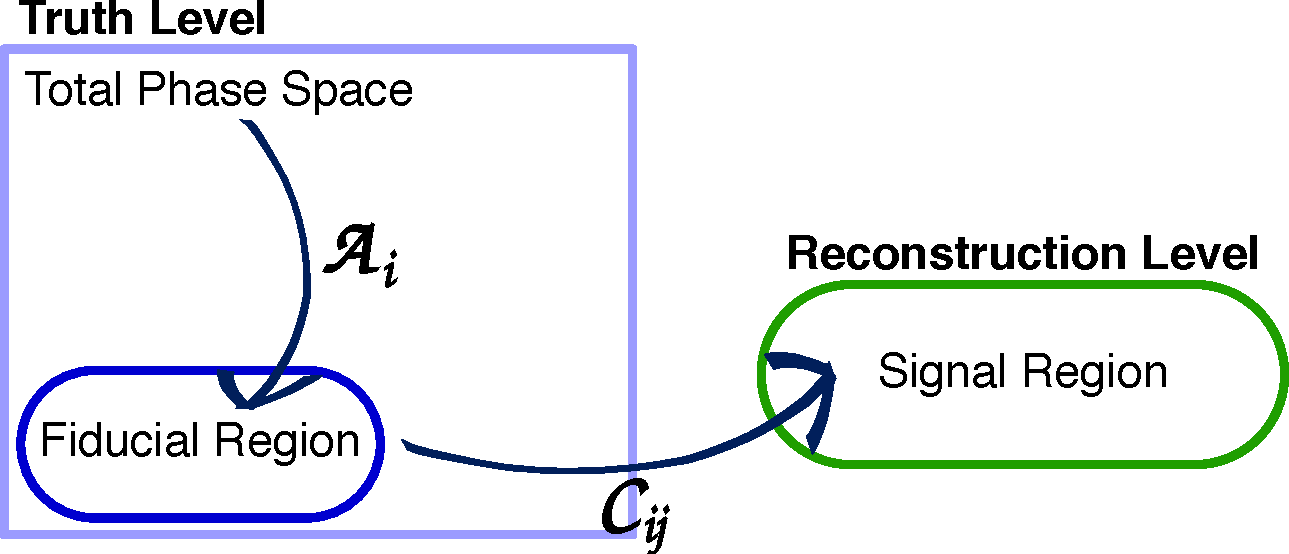
\includegraphics[width=.8\textwidth]{figs/ssww_13tev/xsec/fiducial}
  \caption{Visual representation of the different kinematic regions relevant to the cross section measurement.  The acceptance factor $\mathcal{A}$ converts from the truth level total phase space to the truth level fiducial region, and the efficiency correcction $\mathcal{C}$ translates the fiducial region in to the reconstruction level signal region.}
  \label{fig:ssww13tev_xsec_fiducial_graphic}
\end{figure}

\subsection{Cross section extraction}\label{ssww13tev:xsec_method}
The \ssww EWK fiducial cross section is measured using the signal strength parameter $\mu$ that is determined by the maximum likelihood fit.
This parameter is dependent on the nuisance parameters $\theta$ and can be written explicitly in terms of the measured and theoretical cross sections as:
\begin{equation}
  \mu(\theta) = \frac{\sigma_{\textrm{meas}}^{\textrm{SR}}}{\sigma_{\textrm{theo}}^{\textrm{SR}}}
  \label{eq:ssww13tev_xsec_mu}
\end{equation}

In the simple case with only one bin, the equation for the total number of expected events in the signal region first introduced in Equation~\ref{eq:ssww13tev_xsec_nexp} can be written as:
\begin{equation}
  N_{\textrm{exp}}^{\textrm{SR}}(\theta) = \mu(\theta)\cdot\sigmatottheo\cdot\mathcal{L}\cdot\mathcal{A}\cdot\mathcal{C}(\theta)+N_{\textrm{bkg}}^{\textrm{SR}}(\theta)
  \label{eq:ssww13tev_xsec_nexp_unbinned}
\end{equation}
with the unbinned versions of $\mathcal{A}$ and $\mathcal{C}$ defined in Equations~\ref{eq:ssww13tev_xsec_acceptance} and \ref{eq:ssww13tev_xsec_efficiency}, respectively.

If the measured fiducial cross section is written as:
\begin{equation}
  \sigma_{\textrm{meas}}^{\textrm{fid}} = \mu\cdot\mathcal{A}\cdot\sigmatottheo
\end{equation}
then Equation~\ref{eq:ssww13tev_xsec_nexp_unbinned} can be rearranged to read:
\begin{equation}
  \sigma_{\textrm{meas}}^{\textrm{fid}} = \frac{N_{\textrm{exp}}^{\textrm{SR}}(\theta)-N_{\textrm{bkg}}^{\textrm{SR}}(\theta)}{\mathcal{L}\cdot\mathcal{C}(\theta)}
  \label{eq:ssww13tev_xsec_fid_meas}
\end{equation}
The measured fiducial cross section can finally be rewritten in terms of $\hat{\mu}$, which is the best estimator of the signal strength as extracted from the fit:
\begin{equation}
  \begin{aligned}
    \sigma_{\textrm{meas}}^{\textrm{fid}} &= \hat{\mu}(\theta)\cdot\sigmatottheo\cdot\mathcal{A}\\
    &= \hat{\mu}(\theta)\cdot\sigma_{\textrm{theo}}^{\textrm{fid}}
  \end{aligned}
  \label{eq:ssww13tev_xsec_fid_meas_mu}
\end{equation}

In practice, however, the cross section is not extracted from a single bin, and Equation~\ref{eq:ssww13tev_xsec_nexp_unbinned} becomes:
\begin{equation}
  N_{\textrm{exp}}^{\textrm{SR}}(\theta) = \mu(\theta)\cdot\sigmatottheo\cdot\mathcal{L}\cdot\sum\limits_i\mathcal{A}_i\sum\limits_j\mathcal{C}_{ij}+\sum\limits_j N_{\textrm{bkg},j}^{\textrm{SR}}(\theta)
\end{equation}
for a single channel in truth and reconstruction level $m_{jj}$ bins $i$ and $j$, respectively, where the binned versions of $\mathcal{A}_i$ and $\mathcal{C}_{ij}$ are used.
This equation can be extended to include all the analysis channels by increasing the number of bins $i$ and $j$.
Additionally, it can be shown that Equation~\ref{eq:ssww13tev_xsec_fid_meas_mu} holds for this more complex case as well~\cite{2018.ssww-13tev-atlas-support}, provided care is taken to ensure that all the uncertainties are handled properly.

%\begin{equation}
%  \begin{aligned}
%    N_{\textrm{sig,MC},j} ^{\textrm{SR}}(\theta) &= \sum\limits_i\mathcal{C}_{ij}(\theta)\cdot\mathcal{N}_{\textrm{sig}}^{\textrm{fid}}\\
%    &= \sum\limits_i\mathcal{C}_{ij}(\theta)\big(\mathcal{L}\mathcal{A}_i\sigmatottheo\big)
%  \end{aligned}
%\end{equation}
%then the expected number of signal events in the signal region becomes:
%\begin{equation}
%  N_{\textrm{exp}}^{\textrm{SR}}(\theta) = \mu(\theta)\sum\limits_j N_{\textrm{sig,MC},j}^{\textrm{SR}}(\theta)
%\end{equation}

%\subsection{Results of the cross section measurement}\label{ssww13tev:xsec_results}
%The theoretical fiducial cross section of \ssww EWK production is calculated using \sherpav{2.2.2}.
%The cross section in the total generator phase space is $40.81\pm 0.05\textrm{fb}$, and the fiducial cross section is $2.01\pm 0.02\textrm{fb}$.
%This corresponds to an acceptance factor of $\mathcal{A} = 0.0493\pm 0.0002$.
%Uncertainties on the simulation are estimated using variations of the scale, parton shower, and PDF set.
%The final prediction used in the cross section measurement including uncertainty is:
%\begin{equation}
%  \sigma_{\tt{SHERPA}}^{\textrm{fid}} = 2.01 \pm 0.02(\textrm{stat})~^{+0.29}_{-0.23} (\textrm{scale})~^{+0.16}_{-0.02}(\textrm{parton shower})~^{+0.05}_{-0.03} (\textrm{PDF})~\textrm{fb}
%\end{equation}
